\documentclass[tikz,border=4pt]{standalone}
\usetikzlibrary{arrows.meta,positioning,fit}

\begin{document}
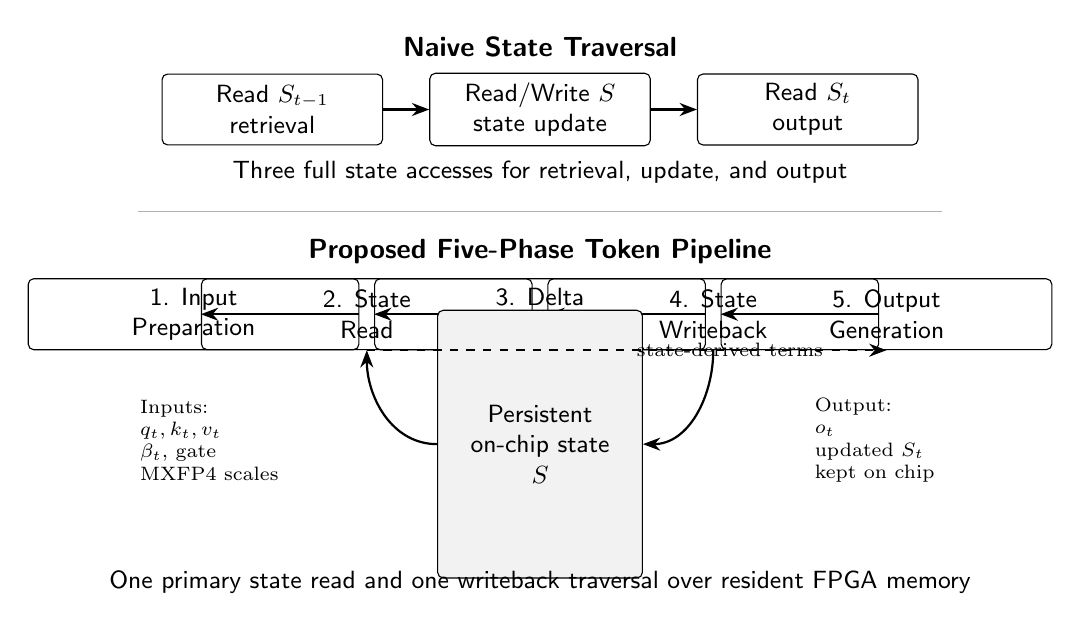
\begin{tikzpicture}[
  font=\sffamily\small,
  box/.style={draw, rounded corners=2pt, align=center, minimum height=9mm, minimum width=28mm},
  widebox/.style={draw, rounded corners=2pt, align=center, minimum height=9mm, minimum width=42mm},
  mem/.style={draw, rounded corners=2pt, align=center, minimum height=34mm, minimum width=26mm, fill=gray!10},
  arrow/.style={-{Stealth[length=2.2mm]}, thick},
  dashedarrow/.style={-{Stealth[length=2.2mm]}, thick, dashed}
]

\node[font=\sffamily\bfseries] at (0, 3.35) {Naive State Traversal};
\node[box] (n1) at (-3.4, 2.55) {Read $S_{t-1}$\\retrieval};
\node[box] (n2) at (0, 2.55) {Read/Write $S$\\state update};
\node[box] (n3) at (3.4, 2.55) {Read $S_t$\\output};
\draw[arrow] (n1) -- (n2);
\draw[arrow] (n2) -- (n3);
\node[align=center] at (0, 1.75) {Three full state accesses for retrieval, update, and output};

\draw[gray!60] (-5.1, 1.25) -- (5.1, 1.25);

\node[font=\sffamily\bfseries] at (0, 0.75) {Proposed Five-Phase Token Pipeline};

\node[widebox] (p1) at (-4.4, -0.05) {1. Input\\Preparation};
\node[widebox] (p2) at (-2.2, -0.05) {2. State\\Read};
\node[widebox] (p3) at (0, -0.05) {3. Delta\\Update};
\node[widebox] (p4) at (2.2, -0.05) {4. State\\Writeback};
\node[widebox] (p5) at (4.4, -0.05) {5. Output\\Generation};

\draw[arrow] (p1) -- (p2);
\draw[arrow] (p2) -- (p3);
\draw[arrow] (p3) -- (p4);
\draw[arrow] (p4) -- (p5);

\node[mem] (state) at (0, -1.7) {Persistent\\on-chip state\\$S$};
\draw[arrow] (state.west) to[out=180,in=270] (p2.south);
\draw[arrow] (p4.south) to[out=270,in=0] (state.east);
\draw[dashedarrow] (p2.south) -- node[right, font=\scriptsize] {state-derived terms} (p5.south);

\node[align=center] at (0, -3.45) {One primary state read and one writeback traversal over resident FPGA memory};

\node[align=left, font=\scriptsize] at (-4.2, -1.65) {
Inputs:\\
$q_t, k_t, v_t$\\
$\beta_t$, gate\\
MXFP4 scales
};

\node[align=left, font=\scriptsize] at (4.25, -1.65) {
Output:\\
$o_t$\\
updated $S_t$\\
kept on chip
};

\end{tikzpicture}
\end{document}
